\subsection{Motivi per fondare una startup}
Ci sono due (possibili) motivi principali per fondare una startup:
\begin{itemize}
 \item successo
 \item guadagno
\end{itemize}

Gli startupper che mirano alla fama cercano di rimanerne il più tempo possibile
``in sella'' alla startup, rimandando l'exit (in quanto la fama calerebbe poi).
Questo significa essere più selettivi negli investitori che vengono scelti e
il guadagno è minore.

All'inizio di un nuovo progetto è necessario decidere quale strategia adottare:
se massimizzare il risultato del progetto e l'aspetto economico o se
massimizzare la fama personale. In base a ciò vanno scelti determinati
investitori, che dovrebbero condividere la stessa visione, altrimenti si
potrebbero verificare situazioni di conflitto.

\subsection{Due tipi di investitori}

Esistono due tipi di investitori:
\begin{itemize}
 \item finanziario
 \item industriale
\end{itemize}
Nel primo caso, investitori come Business Angels o Venture Capital sono coloro
che mirano alla pura speculazione finanziaria. Gli investitori industriali
invece sono quegli investitori (principalmente aziende) che, selezionando un
numero ristretto di start-up, investono in maniera più selettiva dove trovano
un progetto che può essere ritenuto interessante nella loro area di competenza.
Le differenze cruciali tra i due sono:
\begin{itemize}
 \item L'investitore industriale può fornire supporto tecnologico
(partnership). Lo svantaggio è che in questa maniera l'investitore industriale
potrebbe pretendere il controllo della \textit{governance} della startup oppure
essere ingerente nei suoi confronti.
 \item L'investitore finanziario guarda agli aspetti finanziari della startup,
ovvero solo al ritorno monetario. Viceversa, l'investitore industriale è più
tollerante nelle fluttuazioni del successo che può avere l'operazione e non è
interessato solamente ai risultati finanziari, ma anche a quelli
tecnici/industriali.
 \item L'obiettivo finale dei due investitori è molto diverso. Il finanziario
mira solamente all'exit finale. L'investitore industriale potrebbe non voler
l'exit ma addirittura mirare al consolidamento interno del gruppo, ovvero
a ottenere la maggioranza delle quote, facendola entrare nel gruppo aziendale.
\end{itemize}

Per un founder con l'investitore industriale si è già trovato l'exit finale.
Questa strada è ottima come scelta, ma preclude il fatto di avere investitori
finanziari. Si ha quindi di fatto, una scelta esclusiva.
È possibile che ci sia anche una soluzione mista, ma questa può portare a
problemi: infatti se gli investitori sono misti quelli finanziari si potrebbero
ritrovare con dei capitali bloccati che non saranno in grado di recuperare con
un exit. In questo caso, si rischia che l'investitore finanziario trovi accordi
con quello industriale per farlo arrivare fino al 51\% delle quote. In questo
caso, sarà il fondatore stesso ad avere il suo capitale bloccato. La soluzione
quindi è quella di trovare un accordo di vendita con l'investitore industriale
dove si finisce per vedere la maggior parte delle quote (mantenendo solo, per
esempio, il 5\% totale). In questo caso sarà possibile effettuare l'exit con
maggior successo e capitalizzare.

Come si può valutare la propria startup? Di base non è semplice. Le vendite di
quota delle startup dovrebbero essere ampie all'inizio, per poi diminuire man
mano\footnote{Un andamento contrario può essere visto come un fatto negativo da
parte del mercato.}.

\textbf{Golden paracadute}: quanto il proprietario di un'azienda cambia, è a
totale discrezione dei nuovi ``padroni'' decidere se mantenere il corrente
amministratore delegato o cambiarlo con uno nuovo. Per evitare questo è
importante verificare le clausole, ovvero settare un \textit{paracadute d'oro},
in cui si settano delle condizione di assunzione per tot. anni oppure si
stabilisce una liquidazione cospicua al termine dell'incarico.

\chapter{Brand}

Come nella moda, anche nel mondo della tecnologia esistono i \textbf{trend}
(mode). Essi oscillano e si muovono nel tempo.

Quali sono le difficoltà lato startupper e lato sviluppatori? Si tratta di
capire le necessità del periodo per ottenere dei ritorni.

Ci sono diverse modalità per capire quando investire.

La \textit{Gartner}, azienda multinazionale per l'analisi del mercato e
consulenza aziendale, presenta un approccio orientato alle tecnologie. Tra gli
strumenti che mette a disposizione è presente l'\textbf{hype cycle}.
Si è notato che tutte le tecnologie tendono a percorrere un andamento come
descritto in figura \ref{fig:hypecycle}.

\begin{figure}[H]
\centering
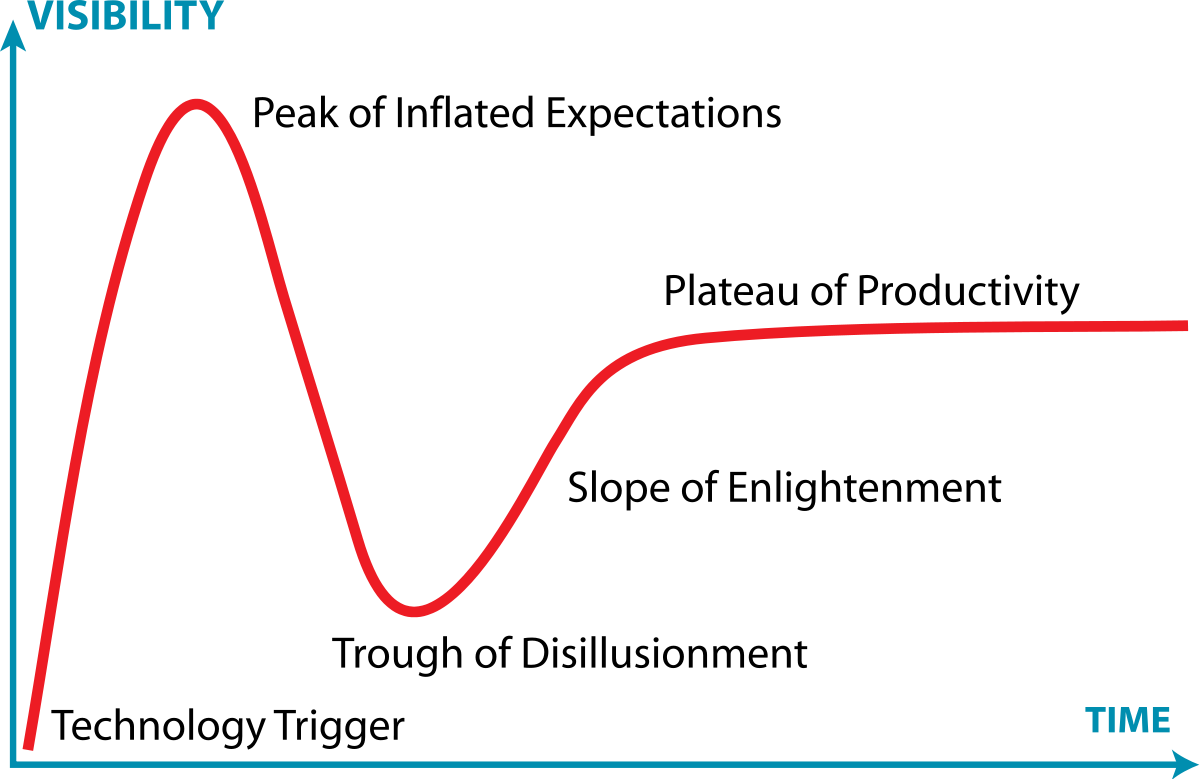
\includegraphics[scale=0.25]{hypecycle.png}
\caption{Hype Cycle - maturità, adozione e applicazione di specifiche
tecnologie.}
\label{fig:hypecycle}
\end{figure}

Le ordinate del grafico rappresentano la visibilità che la tecnologia ha,
mentre le ascisse ne rappresentano la maturità.
Il grafico è diviso in un percorso in cui tutte le tecnologie partono con
visibilità 0 per poi arrivare al picco dell'infatuazione in cui sembra che
quella tecnologia sia necessaria quasi sempre e non se ne possa fare a meno,
per poi arrivare alla delusione delle aspettative stesse.
A questo punto la tecnologia sparisce dal mercato e dai media per poi crescere
di nuovo e raggiungere un certo livello sul quale stabilizzarsi.

Alla nascita di una tecnologia la capacità di adozione è molto minore rispetto
alla visibilità ottenuta grazie ai media.

\paragraph*{Cicli di vita dei prodotti} I prodotti hanno dei specifici cicli di
vita, il cui picco di crescita varia in base alla caratteristica del prodotto
stesso: le auto per esempio hanno un ciclo di vita del prodotto più lungo
rispetto a un prodotto tecnologico (ad esempio un'applicazione).

La vita di un prodotto può essere allungata in diverse maniere:
una di queste può essere l'utilizzo di aggiornamenti (nuove versioni,
aggiunte di funzionalità).

Un errore comune è associare la visibilità di un prodotto con il suo ciclo di
vita.

\begin{figure}[H]
\centering
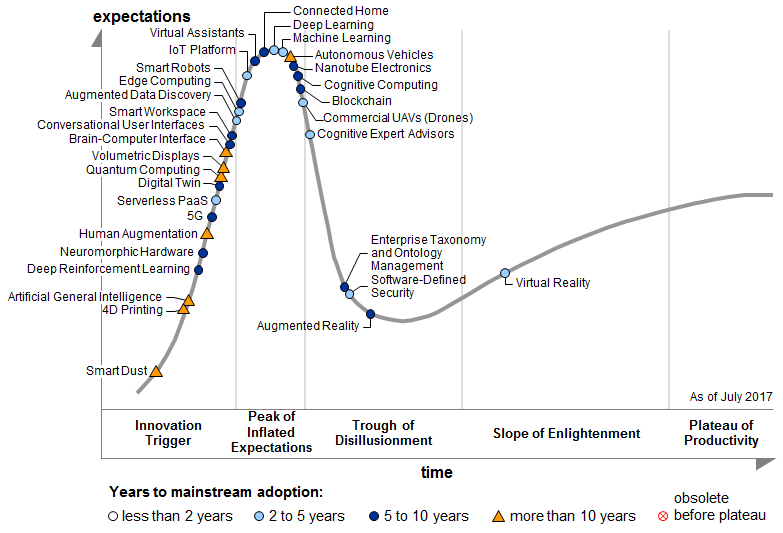
\includegraphics[scale=0.5]{hypecycle2017.png}
\caption{Le tecnologie si muovono lungo l'hype cycle secondo tempi che possono
essere lunghi o brevi (aggiornato al 2017)}
\label{fig:hypecycle}
\end{figure}

\subparagraph*{Gartner priority matrix} Identifica le varie tecnologie e ci
associa il livello di impatto che la tecnologia può avere sulle persone.

\section{Significato di un brand}

Con Brand si fa riferimento sicuramente al logo aziendale, alla sua immagine
(cui fa parte ad esempio il colore), l'insieme di valori, tutti gli aspetti
connessi a quello che per noi rappresenta il marchio che si sta considerando.

\paragraph*{Terminologia} Un brand presenta i seguenti punti caratteristici:
\begin{itemize}
 \item \textbf{Brand image}: tutto ciò che è connesso al brand tramite
l'immagine
 \item \textbf{Brand identity}: ogni brand ha una determinata identità che si
crea volontariamente o che gli viene associata spontaneamente (a volte anche
inconsciamente).
Spostare la brand identity è difficilissimo, richiede un sacco di risorse e
investimenti.
Per questo la reputazione è sempre da tenere sott'occhio, tutt'oggi soprattutto
perché con la diffusione di internet e dei social network è facile diffonderne
un'opinione negativa.
 \item \textbf{Brand reputation}: è la reputazione che un brand ha agli occhi
degli utenti.
Se la reputazione tempo fa era di tipo \textit{broadcast} ovvero andava da un
punto a tutti, oggi è ``distribuita'': viene discussa e parlata tra la gente
 \item \textbf{Brand awareness}: quanto è conosciuto un brand.
È la consapevolezza che ciascuno di noi ha di un brand.
È uno degli asset più importanti che possono avere le aziende storiche e ben
strutturate.
Le aziende serie lavorano che le \textit{personae}, ovvero con quelle persone
di riferimento per il prodotto di vendita, cercandone determinati valori e
caratteristiche.
Più si identificano le caratteristiche più facile è per determinate persone
sposare quelle caratteristiche
 \item \textbf{Brand value}
\end{itemize}
